% 1.1.3. Disk graphs and problem definitions

% For the sake of simplicity, throughout this thesis we often refer to disks and their corre- sponding vertices synonymously. For example, we might simply say ’we create a disk D2 with radius r2 that touches disk D1’ instead of saying ’we create a vertex v2, a correspond- ing disk D2 with radius r2 and an edge between v2 and vertex v1 whose corresponding disk is D1’.
% Let G = (V, E) be a graph. We say that G has a realization as a disk intersection (touching) graph, if there exist a set of disks V and a bijection from V to V such that G = (G,V) is a disk intersection (touching) graph. In this case, we say G realizes G. Let Dv ∈ V be the disk of G corresponding to vertex v for any v ∈ V . A radius assignment for G is a function r : V → R+ that assigns a positive real number to each vertex of G. If the radius of disk Dv ∈ V is equal to r(v) for every v ∈ V , then G is said to respect r. A seed assignment for G is a function σ : V → R2 that assigns a point in the plane to each vertex ofG.Ifσ(v)∈Dv foreveryv∈V,thenGissaidtorespectσ.LetΓbeacombinatorial embedding for G. If G is a disk touching graph and if the cyclic order of disks touched by Dv corresponds to the cyclic order of edges incident to the vertex v for any v ∈ V , then G is said to respect Γ.
% We consider the following family of decision problems, in which the dots (...) are a place- holder for one, multiple or none of the enlisted variants.
% (Unit/ρ-bounded) Disk Intersection/Touching Graph Recognition (with ...): The problem instance is a graph G = (V, E) and the question is whether it is possible to realize G as a (unit/ρ-bounded) disk intersection/touching graph (which respects ...).
% • ... fixed Radii: ... a given radius assignment r for G.
% • ... fixed Embedding: ... a given combinatorial embedding Γ for G. • ... fixed Seeds: ... a given seed assignment σ for G.
% In particular, we consider the following problems:
% • Unit Disk Touching Graph Recognition (UDT)
% • Unit Disk Touching Graph Recognition with fixed Embedding (UDTE)
% • ρ-bounded Disk Touching Graph Recognition (ρ-BDT)
% • Disk Touching Graph Recognition with fixed Radii (DTR)
% • Disk Touching Graph Recognition with fixed Radii and Embedding (DTRE)
% • Disk Touching Graph Recognition with fixed Seeds (DTS)
% • Unit Disk Touching Graph Recognition with fixed Seeds (UDTS)
% • Unit Disk Touching Graph Recognition with fixed Seeds and Embedding (UDTSE)
% 1.2. Related work
% As mentioned in the beginning of this chapter, Koebe’s Theorem [Koe36] implies that the Disk Touching Graph Recognition problem can be solved in linear time. On the other hand, Hlinˇeny ́ and Kratochv ́ıl showed that the Disk Intersection Graph Recognition problem is NP-hard [HK01].
% A result by Breu and Kirkpatrick states that the Unit Disk Intersection/Touching Graph Recognition problems are NP-hard [BK98], implying that the Disk Intersection/Touching Graph Recognition with fixed Radii problems are also N P -hard. There exists some heuris- tics for generating disk touching graphs with fixed radii [Dor96, Ino11] for the application of cartogram generation.
% 6
% Breu and Kirkpatrick generalized their results by showing that the ρ-bounded Disk Inter- section/Touching Graph Recognition problems are NP-hard for any fixed ρ ≥ 1 [BK96]. Alam et al. [AEG+14] argue that for any tree, for any cactus (which is a connected graph in which each edge is contained in at most one cycle), for any k-outerplanar graph with bounded maximum degree and k ∈ O(log n) and for any planar graph with bounded tree- depth there exists a realizing ρ-bounded disk touching graph where ρ is a polynomial in the number of vertices.
% Atienza et al. show that the Disk Touching Graph Recognition with fixed Seeds problem is NP-hard [AdCC+12].








\section{Disk Arrangements}
%Circle packing theorem: For every connected simple planar graph G there is a circle packing in the plane whose intersection graph is (isomorphic to) G.
% A disk D is a region in the plane bounded by a circle. A disk can be uniquely described by its bounding circle’s radius r ∈ R+ and center c ∈ R2. A disk is called closed if it contains the points of its bounding circle and open otherwise. A disk intersection graph G = (G, V) consists of a graph G = (V,E), a set of closed disks V and a bijection from the set of vertices V to V such that two vertices of V are adjacent in G if and only if their corresponding disks in V intersect. A disk touching graph G = (G, V) is a disk intersection graph such that the interiors of the disks in V are pairwise disjoint. The centers of the disks in V together with straight-line segments that connect the centers of all pairs of touching disks induce a planar drawing of G. In a unit disk intersection (touching) graph all disks share one uniform radius. In a ρ-bounded disk intersection (touching) graph the radius of all disks is taken from the interval [1, ρ] for a value ρ ≥ 1. Note, that a 1-bounded disk intersection (touching) graph is a unit disk intersection (touching) graph.
 A \textit{disk arrangement} is a set of interior disjoint disks, $D$, whose centers and radii are defined.  If for any pair of disks in $D$ intersect at a boundary point, they are said to be in contact (kissing).
A \textit{contact graph} $G=(V,E)$ corresponding to a given disk arrangement where there is a bijection $b_V: V \mapsto D$ and a bijection that maps an edge $e_{i,j} \in E$ to an interior disjoint pair of disks $d_i$, $d_j \in D$.
Let $\omega: V \mapsto \bbR^+$ be the \textit{radius assignment} mapping.  $\omega$ assigns a weight to each vertex in $V$.  
$\omega$ \textit{respects radii assignments} of $D$ if for every $v \in V$ such that $b_V(v) = D_v$, $\omega(v)$ is the radius of $D_v$.  
Let $\Pi:V \mapsto \bbr^2$ be that planar mapping of vertices.  $\Pi$ \textit{respects center assignments} of $D$ if for every $v \in V$, $\Pi(v)$ is the center of $D_v$.  
Note that if $\omega$ respects radii assignments, then it can be equivelently said that the linkage $(G,\ell)$ with length assignment $\ell$ also respects radii assignments.  
In this thesis, unless otherwise stated we assume that the contact graph associates to an $\omega$ and $\Pi$ mapping that respect radii and center assignments; we may also interchange contact graph with linkage.
By Koebe's theorem, for every connected simple planar graph $G$, there exists a planar disk arrangement. 



% For the sake of simplicity, throughout this thesis we often refer to disks and their corre- sponding vertices synonymously. For example, we might simply say ’we create a disk D2 with radius r2 that touches disk D1’ instead of saying ’we create a vertex v2, a correspond- ing disk D2 with radius r2 and an edge between v2 and vertex v1 whose corresponding disk is D1’.
% Let G = (V, E) be a graph. We say that G has a realization as a disk intersection (touching) graph, if there exist a set of disks V and a bijection from V to V such that G = (G,V) is a disk intersection (touching) graph. In this case, we say G realizes G. Let Dv ∈ V be the disk of G corresponding to vertex v for any v ∈ V . A radius assignment for G is a function r : V → R+ that assigns a positive real number to each vertex of G. If the radius of disk Dv ∈ V is equal to r(v) for every v ∈ V , then G is said to respect r. A seed assignment for G is a function σ : V → R2 that assigns a point in the plane to each vertex ofG.Ifσ(v)∈Dv foreveryv∈V,thenGissaidtorespectσ.LetΓbeacombinatorial embedding for G. If G is a disk touching graph and if the cyclic order of disks touched by Dv corresponds to the cyclic order of edges incident to the vertex v for any v ∈ V , then G is said to respect Γ.
% %By Koebe's Theorem, every disk arrangement embedded in the plane has a contact graph.
% A \textit{contact graph} represents vertices as interior disjoint disks and by representing edges as as points of intersections (contact), \textit{kissing points} between two disks.  
% The graph corresponding to a given disk arrangement, $\DD$, is said to be the \textit{contact graph}. 
% An ordered disk arrangement preseves the  cyclic order of neighborings disks. 
% %A \it{disk arrangement} is a set, $\DD$, of pairwise interior-disjoint disks in the plane, 
% %$\DD=\left\lbrace C_i \right\rbrace_{i = 1}^n $.
\begin{figure}[!hbtp]
\begin{center}
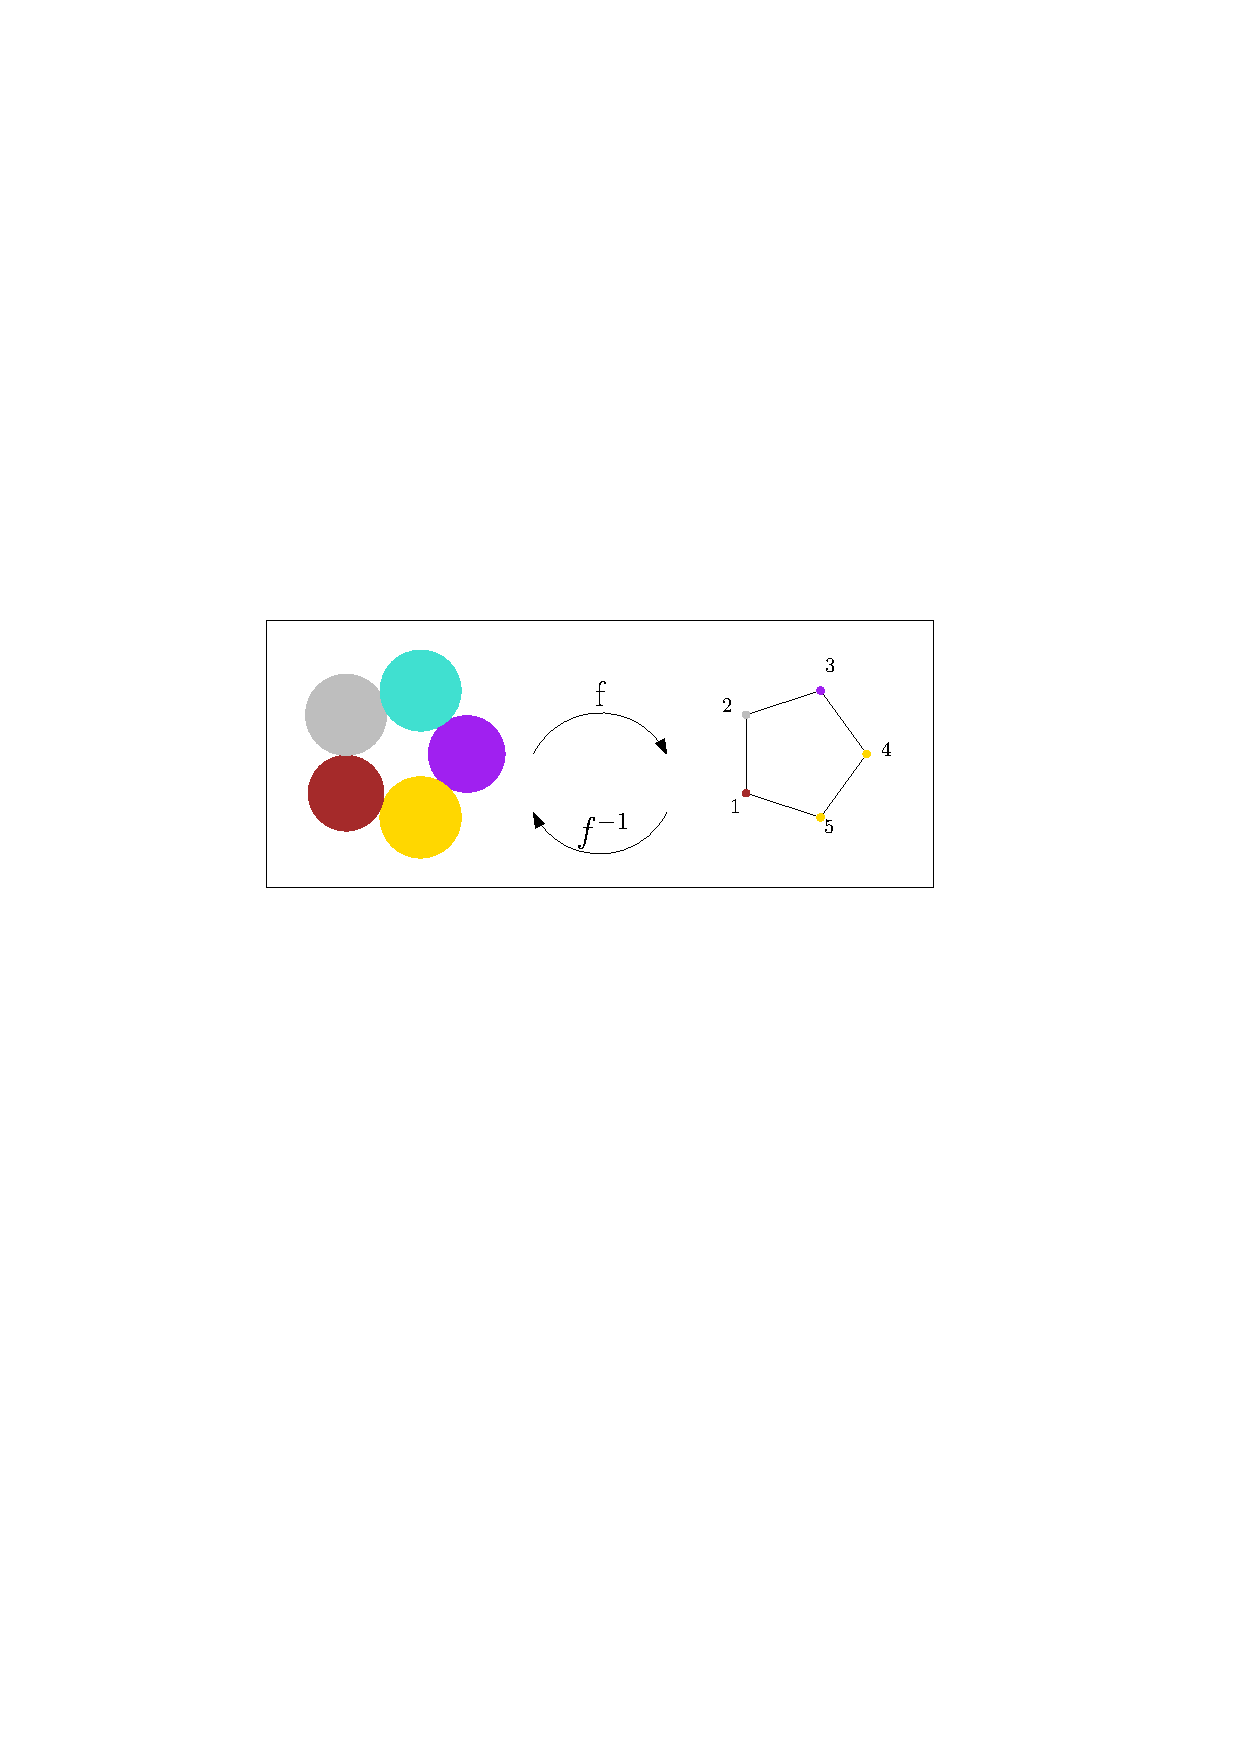
\includegraphics[scale=1]{graphics/diskPackingTheoremExample.pdf}
\end{center} 
\caption{This example represents a disk arrangement transformed to and from its corresponding graph 
$G_2$}
\label{fig:DiskArrangement-1}
\end{figure}

The converse of Koebe's theorem is not true.
It can be a challenge to determine whether a given planar disk arrangement has a contact graph.
The embedding problems for trees and corresponding disk arrangements are as follows:
\begin{prob}[Unordered Realizibility Problem for the Tree]\label{problem:UnorderedTree}
For a tree with positive weighted vertices, it asks whether it is a contact graph of some 
disk arrangement where the radii are equal to the vertex weights.
\end{prob}

\subsection{Disk Packing Confinement Problem}

Given inputs of radii 
By adding constraints to the embeddings of disk arrangements, we can devise realizability problem 
by a volume argument.
\begin{enumerate}%1,2,3,4....
\item Round 1: Start with a disk of unit radius.
\item Round 2: Add two kissing disks, each of diameter 2, that do not intersect with any other 
disk (they 
may kiss other
disk).
\item Round 3 and Higher: For each new kissing disk added, add two more non-intersecting kissing 
disks of diameter 2 to it.
\end{enumerate} 
For each round $i$ we are adding $2^{(i-1)}$ disks, each with an of $\pi$.  The area that 
the disk arrangement is bounded by at round $i$ is a box of length $2\cdot (2\cdot (i-1)+1)$ 
totalling to an area of $(4\cdot i^2 - 4\cdot i + 1)$.  Meanwhile the total area of the disk 
arrangement at round $i$ is $\pi \cdot (2^i - 1)$.  The exponential growth rate of the disk packing 
will exceed its bounded area for sufficiently large $i$.

Figure (\ref{fig:circlePacking-1}) illustrates the iterative problem.  The problem with this is that 
the area in
which is necessary to contain this disk growing disk arrangement will exceed the area needed to 
contain it.
\begin{figure}[H]
\begin{center}
    %add desired spacing between images, e. g. ~, \quad, \qquad etc.
    %(or a blank line to force the subfigure onto a new line)
  \begin{subfigure}[b]{0.24\textwidth}
	  
\includegraphics[width=\textwidth]{graphics/degree2arrangement.pdf}
	  \caption{A disk arrangement with two layers of disks}
	  \label{fig:circlePacking1-1}
  \end{subfigure}
  \begin{subfigure}[b]{0.24\textwidth}
	  
\includegraphics[width=\textwidth]{graphics/degree3arrangement.pdf}
	  \caption{A disk arrangement with three layers of disks}
	  \label{fig:circlePacking1-2}
  \end{subfigure}
  \begin{subfigure}[b]{0.24\textwidth}
	  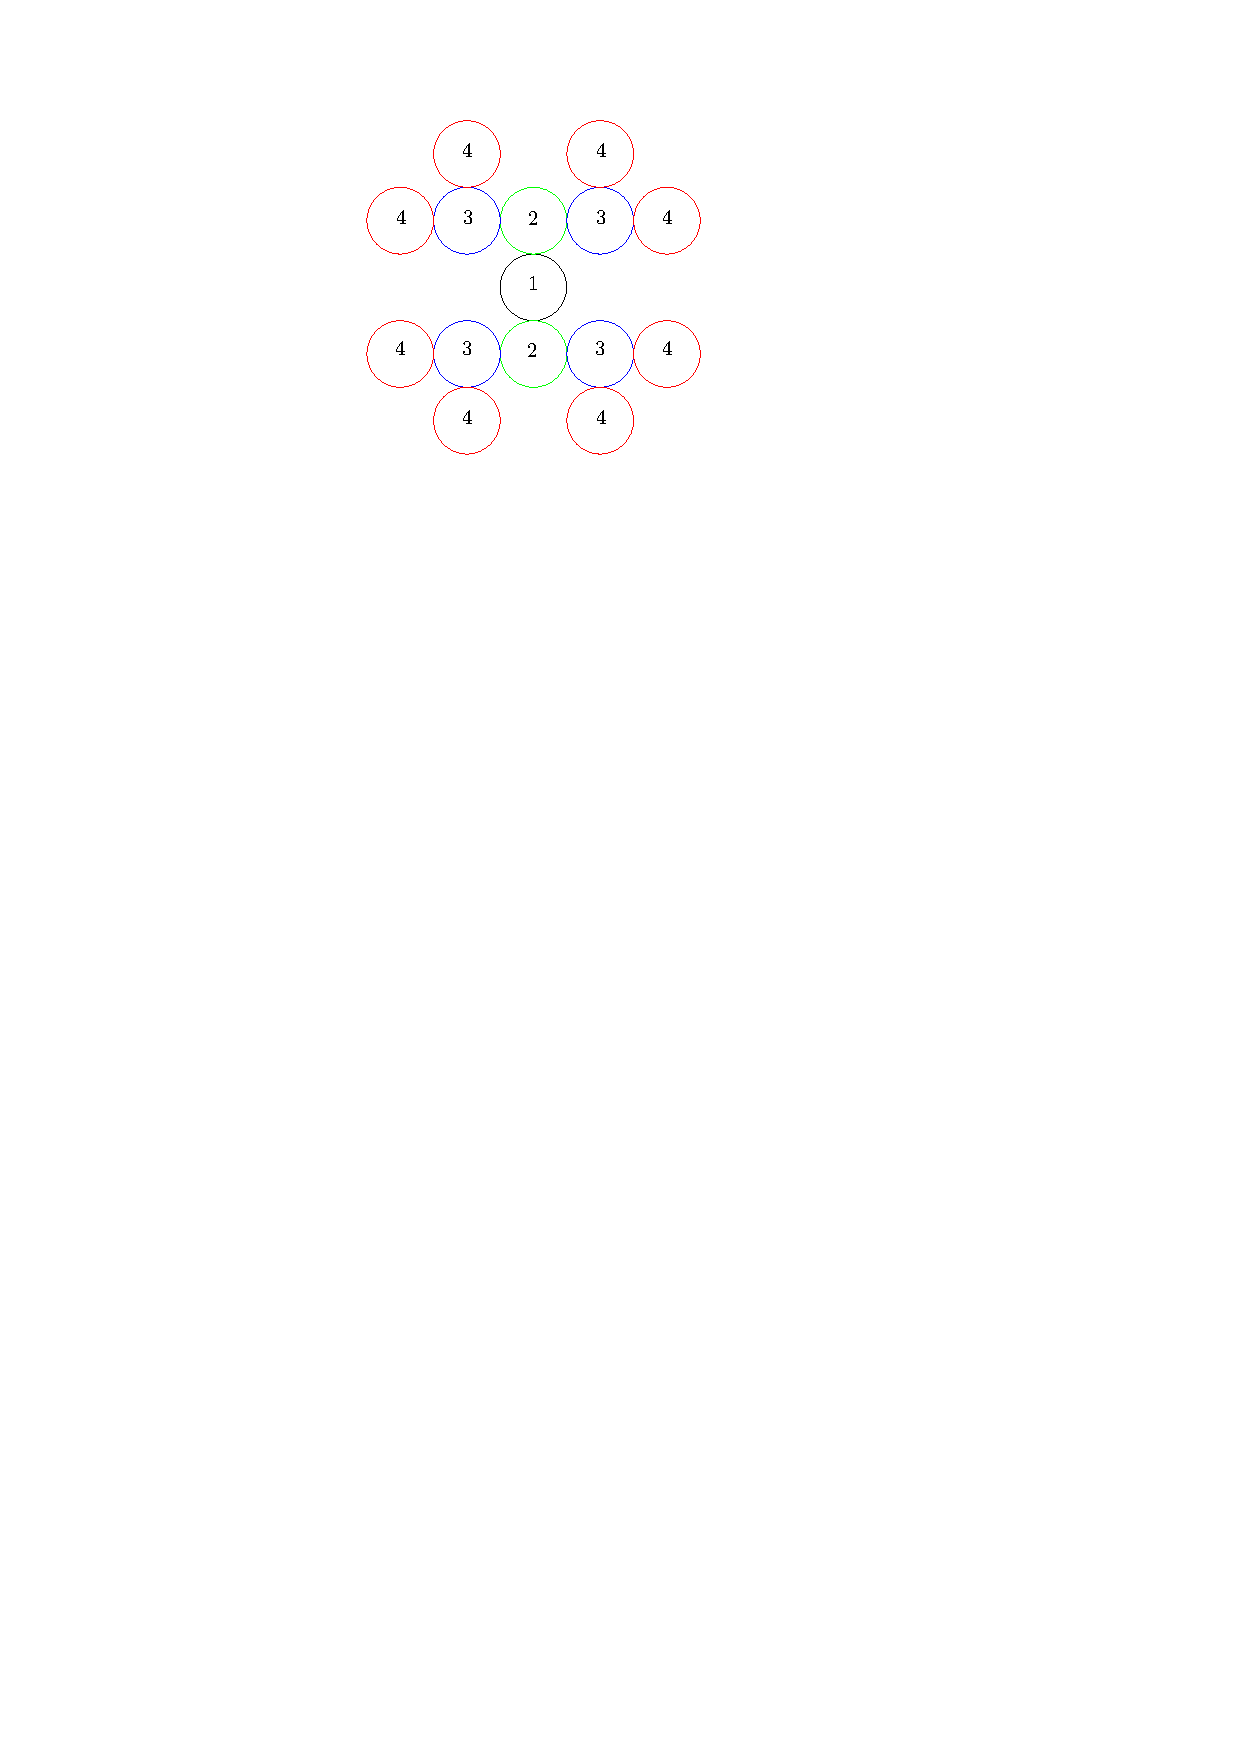
\includegraphics[width=\textwidth]{graphics/degree4arrangement.pdf}
	  \caption{A disk arrangement with four layers of disks}
	  \label{fig:circlePacking1-3}
  \end{subfigure}
  \begin{subfigure}[b]{0.24\textwidth}
	  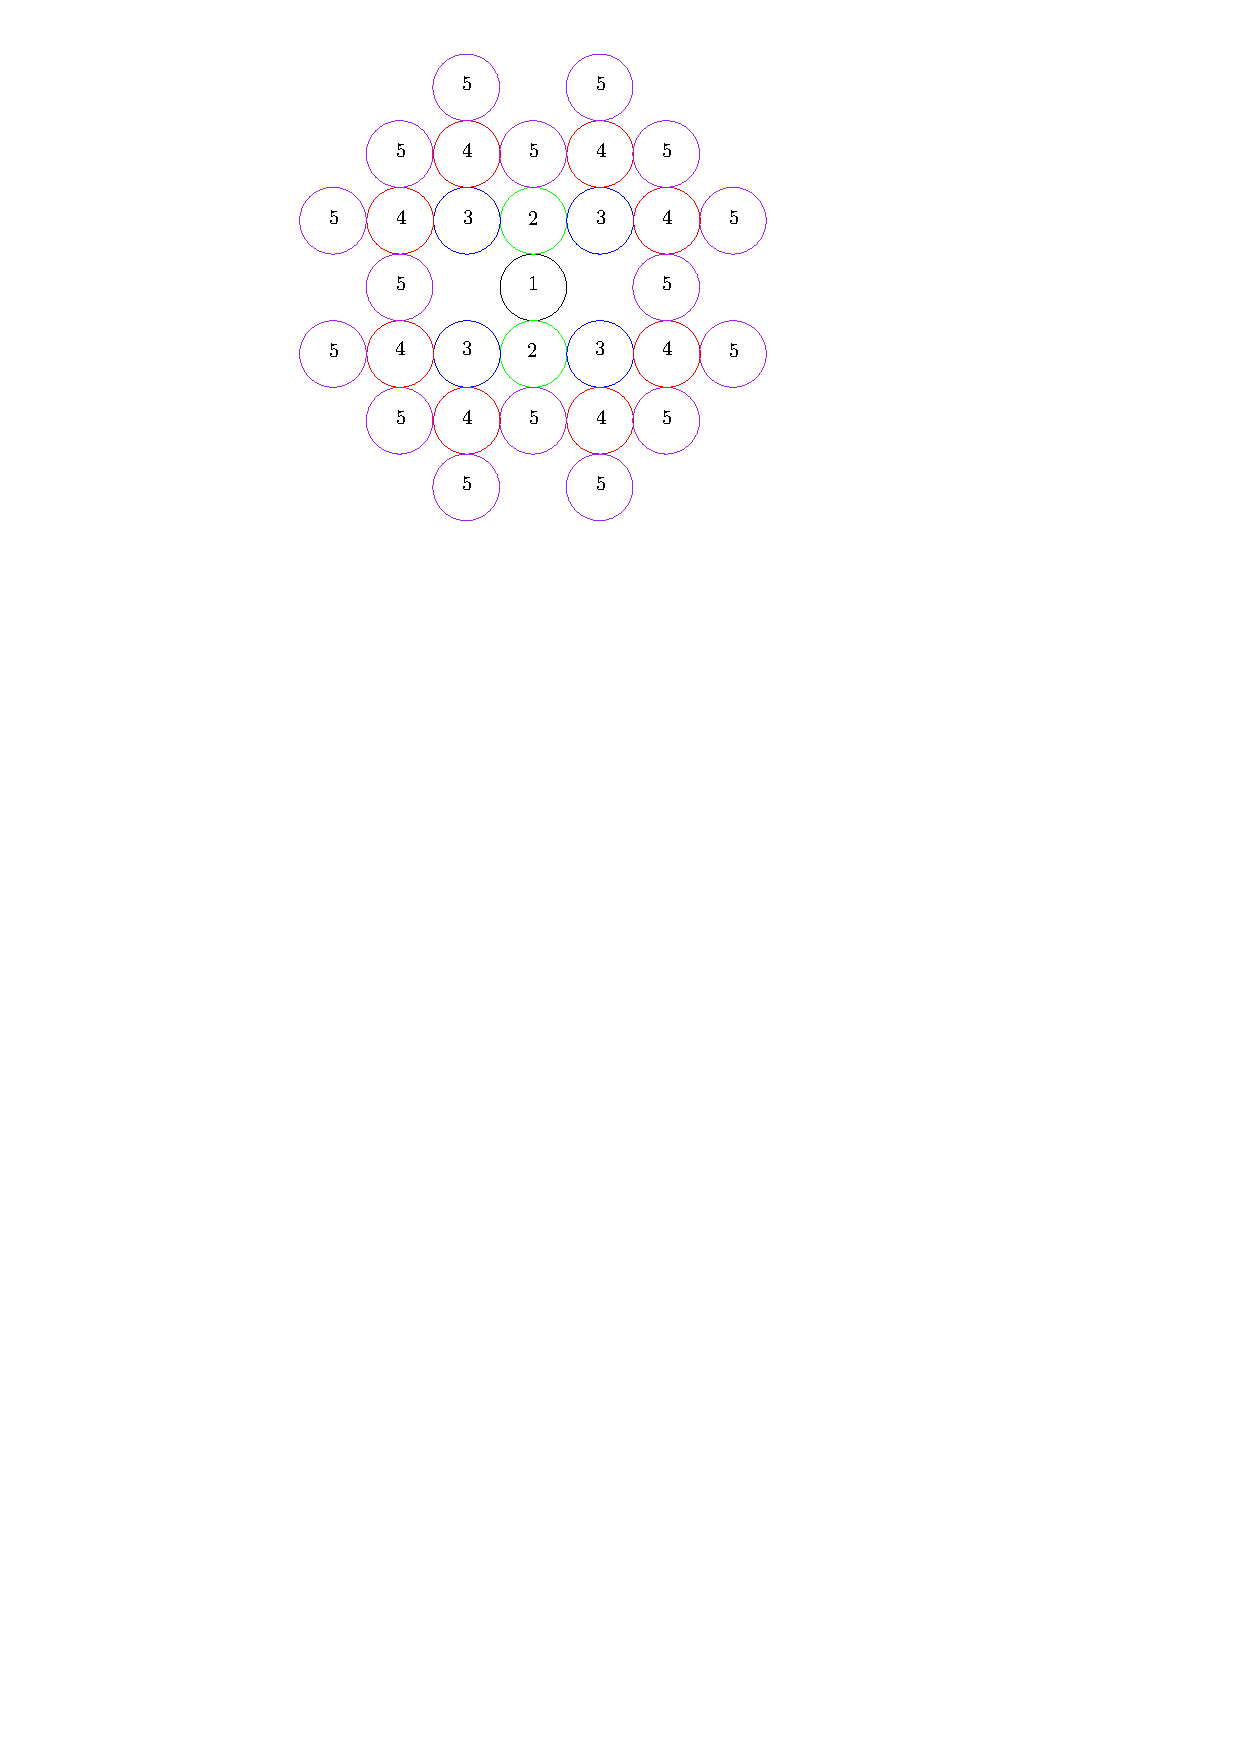
\includegraphics[width=\textwidth]{graphics/degree5arrangement.pdf}
	  \caption{A disk arrangement with five layers of disks}
	  \label{fig:circlePacking1-3}
  \end{subfigure}
\end{center} 
\caption{The gradual growth of disk arrangements by adding two kissing disks to each of the 
previously generated disks.  By continuing this arrangement growth, the space needed to contain the 
kissing disks will exceed the area containing the disk arrangements.}\label{fig:circlePacking-1}
\end{figure}



\begin{prob}[Ordered Realizibility Problem for the Tree]\label{problem:OrderedTree}
For a tree with positive weights for the vertices, it asks whether its corresponding graph is the 
ordered contact graph of some disk arrangement where the radii equal the vertex weights.
\end{prob}
%The corresponding intersection graph of a disk packing is a graph whose vertices are the disks and edges correspond to two disks that contact each other.
% \section{Disk Arrangements}
% It turns out the disk arrangements are an equivalent way to to represent plane graphs.  By 
% representing vertices as interioir disjoint disks and by representing edges as as points of 
% intersections (contact), \textit{kissing 
% points} between two disks.  The graph corresponding to a given disk arrangement, $\DD$, is said to 
% be the \textit{contact graph}. A \it{disk arrangement} is a set, $\DD$, of pairwise 
% interior-disjoint disks in the plane, 
% $\DD=\left\lbrace C_i \right\rbrace_{i = 1}^n $.
% $\left\lbrace C_i \right\rbrace_{i = 1}^n $ such that for any circle $C \in \left\lbrace C_i 
% \right\rbrace_{i = 1}^n$, $C$


% %(fig 1) a disk arrangement
% %(fig 2) an equivalent contact graph to (fig 1)
% A classical result by Thurston and Koebe is that every disk arrangement embedded into the plane had 
% a corresponding plane graph.
% \begin{thm}[\ref{stephenson2005introduction}Disk Packing Theorem]\label{thm2-1}
% For every graph $G$, there is a disk arrangement in the
% plane whose contact graph is isomorphic to $G$.
% \end{thm}

% %add a paragraph with atoms of molecules are modeled with disks and balls of fixed radii. The 
% %if two disks are in contact, then the  distance between their centers  = the sum of the radii
% %conclude: disk arrangements are better models for representing atoms and molecules fixed distance 
% % betweeen atoms
% \begin{prop}
%  For every linkage $L$, there is a disk arrangement in the
% plane whose contact graph is isomorphic to $L$.
% \end{prop}



% \begin{enumerate}%1,2,3,4....
% %\item Introduce the circle packing theorem.
% \item Show the relation between polygonal linkages and disk arrangengements.
% \end{enumerate} 
% % \subsubsection{Ordered Disk Arrangement}
% Suppose we're given a tree. By the disk packing theorem we can ascertain a sense of order for the 
% isomorphic disk packing.  An \textit{ordered disk arrangement} is a rooted tree in which the 
% counter-clockwise ordering of adjacent vertices.
% % 


% The embedding problems for trees and corresponding disk arrangements are as follows:
% \begin{prob}[Unordered Realizibility Problem for the Tree]\label{problem:UnorderedTree}
% For a tree with positive weights for the verticies, it asks whether it is a contact graph of some 
% disk arrangement where the radii are equal to the vertex weights.
% \end{prob}

% \begin{prob}[Ordered Realizibility Problem for the Tree]\label{problem:OrderedTree}
% For a tree with positive weights for the vertices, it asks whether its corresponding graph is the 
% ordered contact graph of some disk arrangement where the radii equal the vertex weights.
% \end{prob}
